% this TeX file provides an awesome example of how TeX will make super 
% awesome tables, at the cost of your of what happens when you try to make a
% table that is very complicated.
% Originally turned in for Dr. Nico's Security Class
\documentclass[11pt]{article}


% Use wide margins, but not quite so wide as fullpage.sty
\marginparwidth 0.5in 
\oddsidemargin 0.25in 
\evensidemargin 0.25in 
\marginparsep 0.25in
\topmargin 0.25in 
\textwidth 6in \textheight 8 in
% That's about enough definitions

% multirow allows you to combine rows in columns
\usepackage{multirow}
% tabularx allows manual tweaking of column width
\usepackage{tabularx}
% longtable does better format for tables that span pages
\usepackage{longtable}
\usepackage{mathtools}
\usepackage{listings}
\usepackage{color}
 
\definecolor{codegreen}{rgb}{0,0.6,0}
\definecolor{codegray}{rgb}{0.5,0.5,0.5}
\definecolor{codepurple}{rgb}{0.58,0,0.82}
\definecolor{backcolour}{rgb}{0.95,0.95,0.92}
 
\lstdefinestyle{mystyle}{
      backgroundcolor=\color{backcolour},   
          commentstyle=\color{codegreen},
              keywordstyle=\color{magenta},
                  numberstyle=\tiny\color{codegray},
                      stringstyle=\color{codepurple},
                          basicstyle=\footnotesize,
                              breakatwhitespace=false,         
                                  breaklines=true,                 
                                      captionpos=b,                    
                                          keepspaces=true,                 
                                              numbers=left,                    
                                                  numbersep=5pt,                  
                                                      showspaces=false,                
                                                          showstringspaces=false,
                                                              showtabs=false,                  
                                                                  tabsize=2
                                                                }


                                                                
                                                                
                                  \lstset{style=mystyle}
\begin{document}
% this is an alternate method of creating a title
%\hfill\vbox{\hbox{Gius, Mark}
%       \hbox{Cpe 456, Section 01}  
%       \hbox{Lab 1}    
%       \hbox{\today}}\par
%
%\bigskip
%\centerline{\Large\bf Lab 1: Security Audit}\par
%\bigskip
\author{Finlay McAfee - s1220880}
\title{Algorithmic Game Theory and Applications - Coursework 1}
\maketitle

\section{}
Let A be the bimatrix defining the 2-player strategic game G:
\begin{equation}
  A = 
  \begin{bmatrix}
    (6, 8) & (2,9) & (3,8) & (2,8) \\
    (0, 5) & (2,3) & (2,6) & (8,4) \\
    (7, 0) & (2,7) & (4,4) & (4,3) \\
    (2, 3) & (5,3) & (2,5) & (5,4) \\
  \end{bmatrix}
\end{equation}
\subsection{Elimination}
First we can eliminate the strongly dominated pure strategies from A to solve an equivalent but easier game.

For a pure strategy $x_i \in X_i$ to be strictly dominated there must exist another strategy $x'_i$ such that, for all $x_{-i} \in X_{-i}$:
\begin{equation}
  U_i(x_{-i};x'_i) > U_i(x_{-i};x_i)
\end{equation}

Note that this $x'_i$ does not need to be a pure strategy. There are no pure strategies that strictly dominate any others in this game. But there are mixed strategies that dominate pure strategies.

Take $x'_2$ to be $(0,\frac{1}{4},\frac{3}{4},0)$. This mixed strategy strictly dominates $\pi_{2,1}$ and $\pi_{2,4}$ as:

\begin{align}
  U_2(\pi_{1,1};x'_2) = 8.25 \\
  U_2(\pi_{1,2};x'_2) = 5.25 \\
  U_2(\pi_{1,3};x'_2) = 4.75 \\
  U_2(\pi_{1,4};x'_2) = 4.5
\end{align}

Hence we can eliminate columns 1 and 4 from A:

\begin{equation}
  A' = 
  \begin{bmatrix}
    (2,9) & (3,8) \\
    (2,3) & (2,6) \\
    (2,7) & (4,4) \\
    (5,3) & (2,5)
  \end{bmatrix}
\end{equation}

By the same method we can choose $x'_1$ to be $(0,0,\frac{2}{3},\frac{1}{3})$ which strictly dominates $\pi_{1,1}$ and $\pi_{1,2}$.

Therefore we can solve the following reduced matrix to find all Nash Equilibrium for the game G:
\begin{equation}
  A'' = 
  \begin{bmatrix}
    (2,7) & (4,4) \\
    (5,3) & (2,5)
  \end{bmatrix}
\end{equation}

\subsection{Computing NE}

It is clear by inspection that there are no pure Nash Equilibria. This is because, for every profile of pure strategies, there is always a player that is better off unilaterally switching to the other available pure strategy. By the definition of a Nash Equilibrium, this rules out pure NEs for the game G. By a similar argument there are no NE where one player plays a pure strategy and the other a mixed. However Nash's theorem tells us that a NE does exist, and as it must be a mixed NE, both players must play each strategy with positive probability. This means that each pure strategy, for both players, is a best response in a NE, by the Useful Corollary to Nash's Theorem.

Let $x^*_1(1)$, the probability of player 1 playing the strategy 1 in the NE, be $a$ and $x^*_1(2)$ be $1-a$. Let $x^*_2(1)$ be $b$ and $x^*_2(2)$ be $1-b$.

\begin{align}
  U^*_1(x^*_{-1};\pi_{1,1}) = U^*_1(x^*_{-1};\pi_{1,2}) \\
  2b + 4(1-b) = 5b + 2(1-b) \\
  4 - 2b = 2 + 3b \\
  b = \frac{2}{5}
\end{align}

Hence $x^*_2 = (\frac{2}{5}, \frac{3}{5})$, or $(0,\frac{2}{5}, \frac{3}{5}, 0)$ under the original game.

\begin{align}
  U^*_2(x^*_{-1};\pi_{2,1}) = U^*_2(x^*_{-1};\pi_{2,2}) \\
  7a + 3(1-a) = 4a + 5(1-a) \\
  3 + 4a = 5 - a \\
  a = \frac{2}{5}
\end{align}

Hence $x^*_1 = x^*_2$ (under the reduced game) and the profile of the NE for game G is 

\begin{equation}
  [(0,0,\frac{2}{5}, \frac{3}{5}), (0,\frac{2}{5}, \frac{3}{5}, 0)]
\end{equation}
As there was no loss of generality in these assumptions, it is clear that this is the only NE that exists for this game.

\section{}

The LP corresponding to the given 2-player zero sum game can be specified by:

\begin{flalign*}
  \textbf{maximise} \quad v \\
  \textbf{subject to:} \\
  v - (7x_1 + 2x_2 + 6x_3 + 5x_4 + 2x_5) \leq 0 \\
  v - (x_1 + 6x_2 + 3x_3 + 5x_4 + 8x_5) \leq 0 \\
  v - (6x_1 + 8x_2 + 8x_3 + 4x_4 + 2x_5) \leq 0 \\
  v - (4x_1 + 3x_2 + 3x_3 + 7x_4 + 8x_5) \leq 0 \\
  v - (2x_1 + 5x_2 + 4x_3 + 4x_4 + 9x_5) \leq 0 \\
  x_1 + x_2 + x_3 + x_4 + x_5 = 1 \\
  x_i \geq 0 \quad \text{for} \quad j = 1,...,5
\end{flalign*}

This was computed using the {\tt linprog} function in {\tt MATLAB} in the following manner:

Constraints 1,...,5 were encoded in the form $A\textbf{x} \leq \textbf{b}$ where:

\begin{align}
  \textbf{b} = \textbf{0} \\
  A = 
  \begin{bmatrix}
  1 & -7 & -2 & -6 & -5 & -2 \\
  1 & -1 & -6 & -3 & -5 & -8 \\
  1 & -6 & -8 & -8 & -4 & -2 \\
  1 & -4 & -3 & -3 & -7 & -8 \\
  1 & -2 & -5 & -4 & -4 & -9
  \end{bmatrix}
\end{align}

Constraint 6 was encoded in the form:

\begin{align}
  \text{beq} = 1 \\
  Aeq = [0, 1, 1, 1, 1, 1]
\end{align}

And Contraint 7 was encoded as lower bounds for the variables $x_1, ..., x_5$

The program produced the following results:

\begin{align}
  v = 4.8333 \\
  x_1 = 0 \\
  x_2 = 0 \\
  x_3 = 0.3333 \\
  x_4 = 0.5 \\
  x_5 = 0.1667
\end{align}

Hence the minimax value of this game is 4.8333 and the optimal strategy for player 1 is $x^*_1 = (0,0,0.3333,0.5,0.1667)$.

The variables of the dual of the linear program can be interpreted as the optimal strategy for player 2.

\begin{flalign*}
  \textbf{minimise} \quad u \\
  \textbf{subject to:} \\
  u - (7y_1 + 1y_2 + 6y_3 + 4y_4 + 2y_5) \leq 0 \\
  u - (2y_1 + 6y_2 + 8y_3 + 3y_4 + 5y_5) \leq 0 \\
  u - (6y_1 + 3y_2 + 8y_3 + 3y_4 + 4y_5) \leq 0 \\
  u - (5y_1 + 5y_2 + 4y_3 + 7y_4 + 4y_5) \leq 0 \\
  u - (2y_1 + 8y_2 + 2y_3 + 8y_4 + 9y_5) \leq 0 \\
  y_1 + y_2 + y_3 + y_4 + y_5 = 1 \\
  y_i \geq 0 \quad \text{for} \quad j = 1,...,5
\end{flalign*}

Computing this dual LP using {\tt MATLAB} gives the following values:

\begin{align}
  u = 4.8333 \\
  y_1 = 0.5556 \\
  y_2 = 0.2778 \\
  y_3 = 0 \\
  y_4 = 0 \\
  y_5 = 0.1667
\end{align}

Hence player 2's optimal strategy is $x^*_2 = (0.5556,0.2778,0,0,0.1667)$.

\section{}

\begin{equation}
  \begin{bmatrix}
    1 & -1 \\
    -1 & 1
  \end{bmatrix}
\end{equation}

\subsection*{(a)}

The unique NE of the Matching Pennies game is given by $x^* = [(0.5,0.5),(0.5,0.5)]$

\subsection*{(b)}

The experimental method was chosen for showing (but not proving) that the statistical mixed profile of this game approaches the above NE.

The tie breaking rule used was an arbitrary artifact of the implementation. Player 1 will chose tails in a tie and player 2 will chose heads.

Figures 1-4 show the estimated probability of the other player choosing the heads strategy under the statistical mixed strategy, for both players under all possible starting strategies.

Here follows the python implementation of the Matching Pennies Game:

\lstinputlisting[language=Python, caption=question3.py]
{question3.py}

\begin{figure}[h]
  \caption{Player 1: Started with Heads, Player 2: Started with Heads}
  \centering
  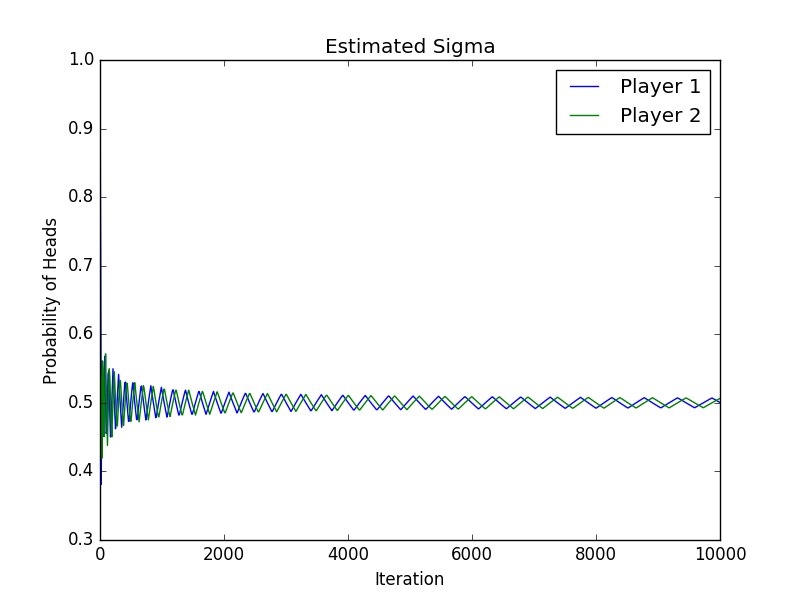
\includegraphics[width=0.5\textwidth]{hh}
\end{figure}

\begin{figure}[h]
  \caption{Player 1: Started with Heads, Player 2: Started with Tails}
  \centering
  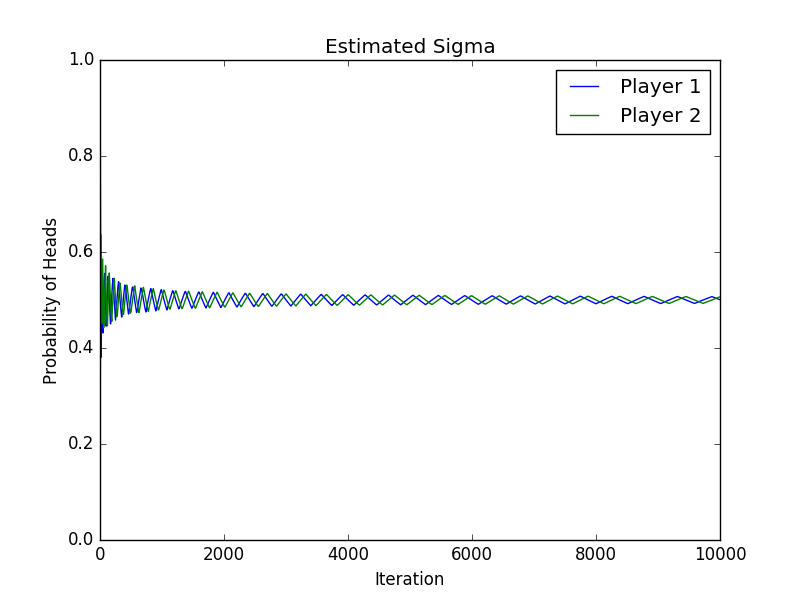
\includegraphics[width=0.5\textwidth]{ht}
\end{figure}

\begin{figure}[h]
  \caption{Player 1: Started with Tails, Player 2: Started with Heads}
  \centering
  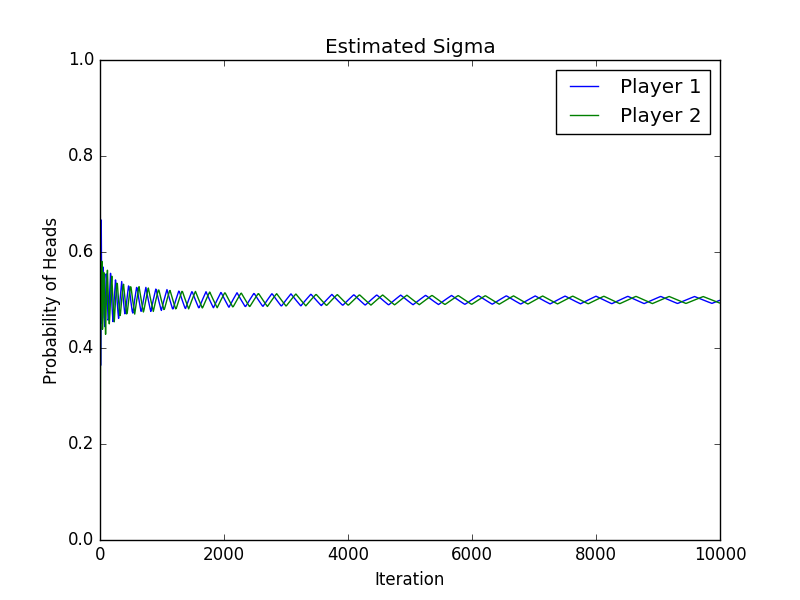
\includegraphics[width=0.5\textwidth]{th}
\end{figure}

\begin{figure}[h]
  \caption{Player 1: Started with Tails, Player 2: Started with Tails}
  \centering
  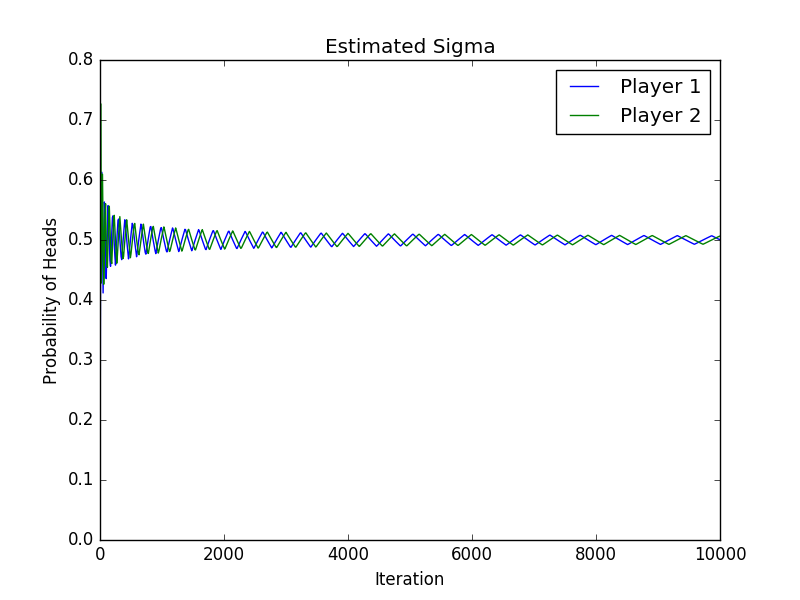
\includegraphics[width=0.5\textwidth]{tt}
\end{figure}

\section{}

\subsection*{(a)}

To show that there exists a strategy $x_1$ for player 1 that, if commited to, will increase their payoff to strictly greater than 6, first note that player 2 will respond with pure strategy 2 whenever $x_1(2) > x_1(1)$, as this will maximise their expected payoff. In the case of $x_1 = (0.25, 0.75)$ the expected payoff is player 2 chooses strategy 1 will be 2.25 and 2.75 for strategy 2. Now also note that, given player 2 is playing pure strategy 2, the expected payoff for player 1 will always be strictly greater than 6 by playing strategy 1 with non-zero probability, hence all mixed strategies $$x_1 \quad s.t. \quad x_1(1) > 0, x_1(2) > x_1(1)$$ achieve a payoff $> 6$.

\subsection*{(b)}

Based on the above reasoning and the new information about player 2's 'kind' strategy in the indifferent case, it is clear that the mixed strategy that maximises player 1's payoff is the one where he plays strategy 1 with the highest probability under the new conditions $$x_1 \quad s.t. \quad x_1(1) > 0, x_1(2) \geq x_1(1)$$, which is $x_1 = (0.5, 0.5)$.

\subsection*{(c)}



\end{document}
